\documentclass[../PiTest.tex]{subfiles}

\begin{document}

\section{Project definition}

    The project definition will be splitted in two sections, describing the server and on the client.

    \subsection{Server}
    The server application, from now on \pitest, is installed on the Operating System of the board and needs NodeJS to work.

    \subsubsection{Class diagram}
    The following is an high level diagram of the architecture of \pitest.
    
    \begin{figure}[!h]
        \centering
        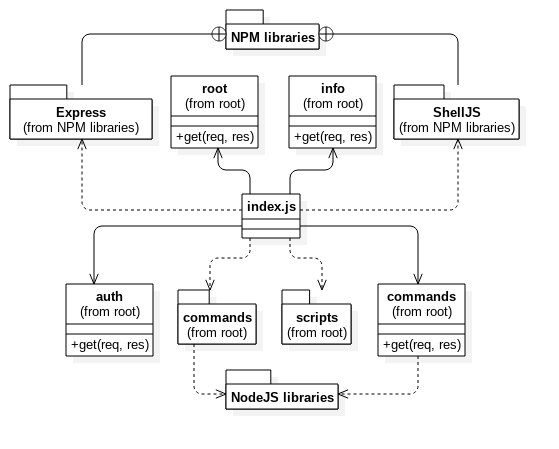
\includegraphics[width=\textwidth+1cm, height=10cm, keepaspectratio]{\detokenize{UML/png/Model__Achitecture Diagram_4.png}}
        \caption{High level architectural diagram}
    \end{figure}

    \clearpage



    \subsection{Client}


\end{document}